\let\negmedspace\undefined
\let\negthickspace\undefined
\documentclass[journal]{IEEEtran}
\usepackage[a5paper, margin=10mm, onecolumn]{geometry}
%\usepackage{lmodern} % Ensure lmodern is loaded for pdflatex
\usepackage{tfrupee} % Include tfrupee package

\setlength{\headheight}{1cm} % Set the height of the header box
\setlength{\headsep}{0mm}     % Set the distance between the header box and the top of the text

\usepackage{gvv-book}
\usepackage{gvv}
\usepackage{cite}
\usepackage{amsmath,amssymb,amsfonts,amsthm}
\usepackage{algorithmic}
\usepackage{graphicx}
\usepackage{textcomp}
\usepackage{xcolor}
\usepackage{txfonts}
\usepackage{listings}
\usepackage{enumitem}
\usepackage{mathtools}
\usepackage{gensymb}
\usepackage{comment}
\usepackage[breaklinks=true]{hyperref}
\usepackage{tkz-euclide} 
\usepackage{listings}
\def\inputGnumericTable{}                                 
\usepackage[latin1]{inputenc}                                
\usepackage{color}                                            
\usepackage{array}                                            
\usepackage{longtable}                                       
\usepackage{calc}                                             
\usepackage{multirow}                                         
\usepackage{hhline}                                           
\usepackage{ifthen}                                           
\usepackage{lscape}
\begin{document}

\bibliographystyle{IEEEtran}
\vspace{3cm}

\title{1.11.14}
\author{AI25BTECH11012 - GARIGE UNNATHI}
% \maketitle
% \newpage
% \bigskip
{\let\newpage\relax\maketitle}


\renewcommand{\thefigure}{\theenumi}
\renewcommand{\thetable}{\theenumi}
\setlength{\intextsep}{10pt} % Space between text and floats


\numberwithin{equation}{enumi}
\numberwithin{figure}{enumi}
\renewcommand{\thetable}{\theenumi}


\textbf{Question}:\\
If $\vec{a} = 4\hat{i} - \hat{j} + \hat{k}$ and $\vec{b} = 2\hat{i} - 2\hat{j} + \hat{k}$, 
then find a unit vector parallel to the vector $\vec{a} + \vec{b}$.
 
\textbf{Solution: }

 \begin{table}[h!]    
      \centering
      

      \caption{Variables Used}
      \label{}
    \end{table}

The unit vector in the direction of the vector  $\vec{a} + \vec{b}$ is given by the equation :

 \begin{align*}
\frac{\vec{a}+\vec{b}}{\lVert \vec{a}+\vec{b} \rVert}
\end{align*}


\begin{align}
   \vec{a}+\vec{b} = \myvec{4 \\ -1 \\ 1} + \myvec{2 \\ -2 \\ 1} = \myvec{6 \\ -3 \\ 2}
\end{align}


\begin{align}
   \frac{\vec{a}+\vec{b}}{\lVert \vec{a}+\vec{b} \rVert} = \frac{1}{7} \myvec{6 \\ -3 \\ 2}
\end{align}


\begin{align}
= \myvec{\frac{6}{7} \\ -\frac{3}{7} \\ \frac{2}{7}}
\end{align}

Hence the unit vector in the direction of the vector $\vec{a} + \vec{b}$ is $\myvec{\frac{6}{7} \\ -\frac{3}{7} \\ \frac{2}{7}}$ = $\frac{6}{7}\hat{i} - \frac{3}{7}\hat{j} + \frac{2}{7}\hat{k}$ 

\begin{figure}[h!]
   \centering
   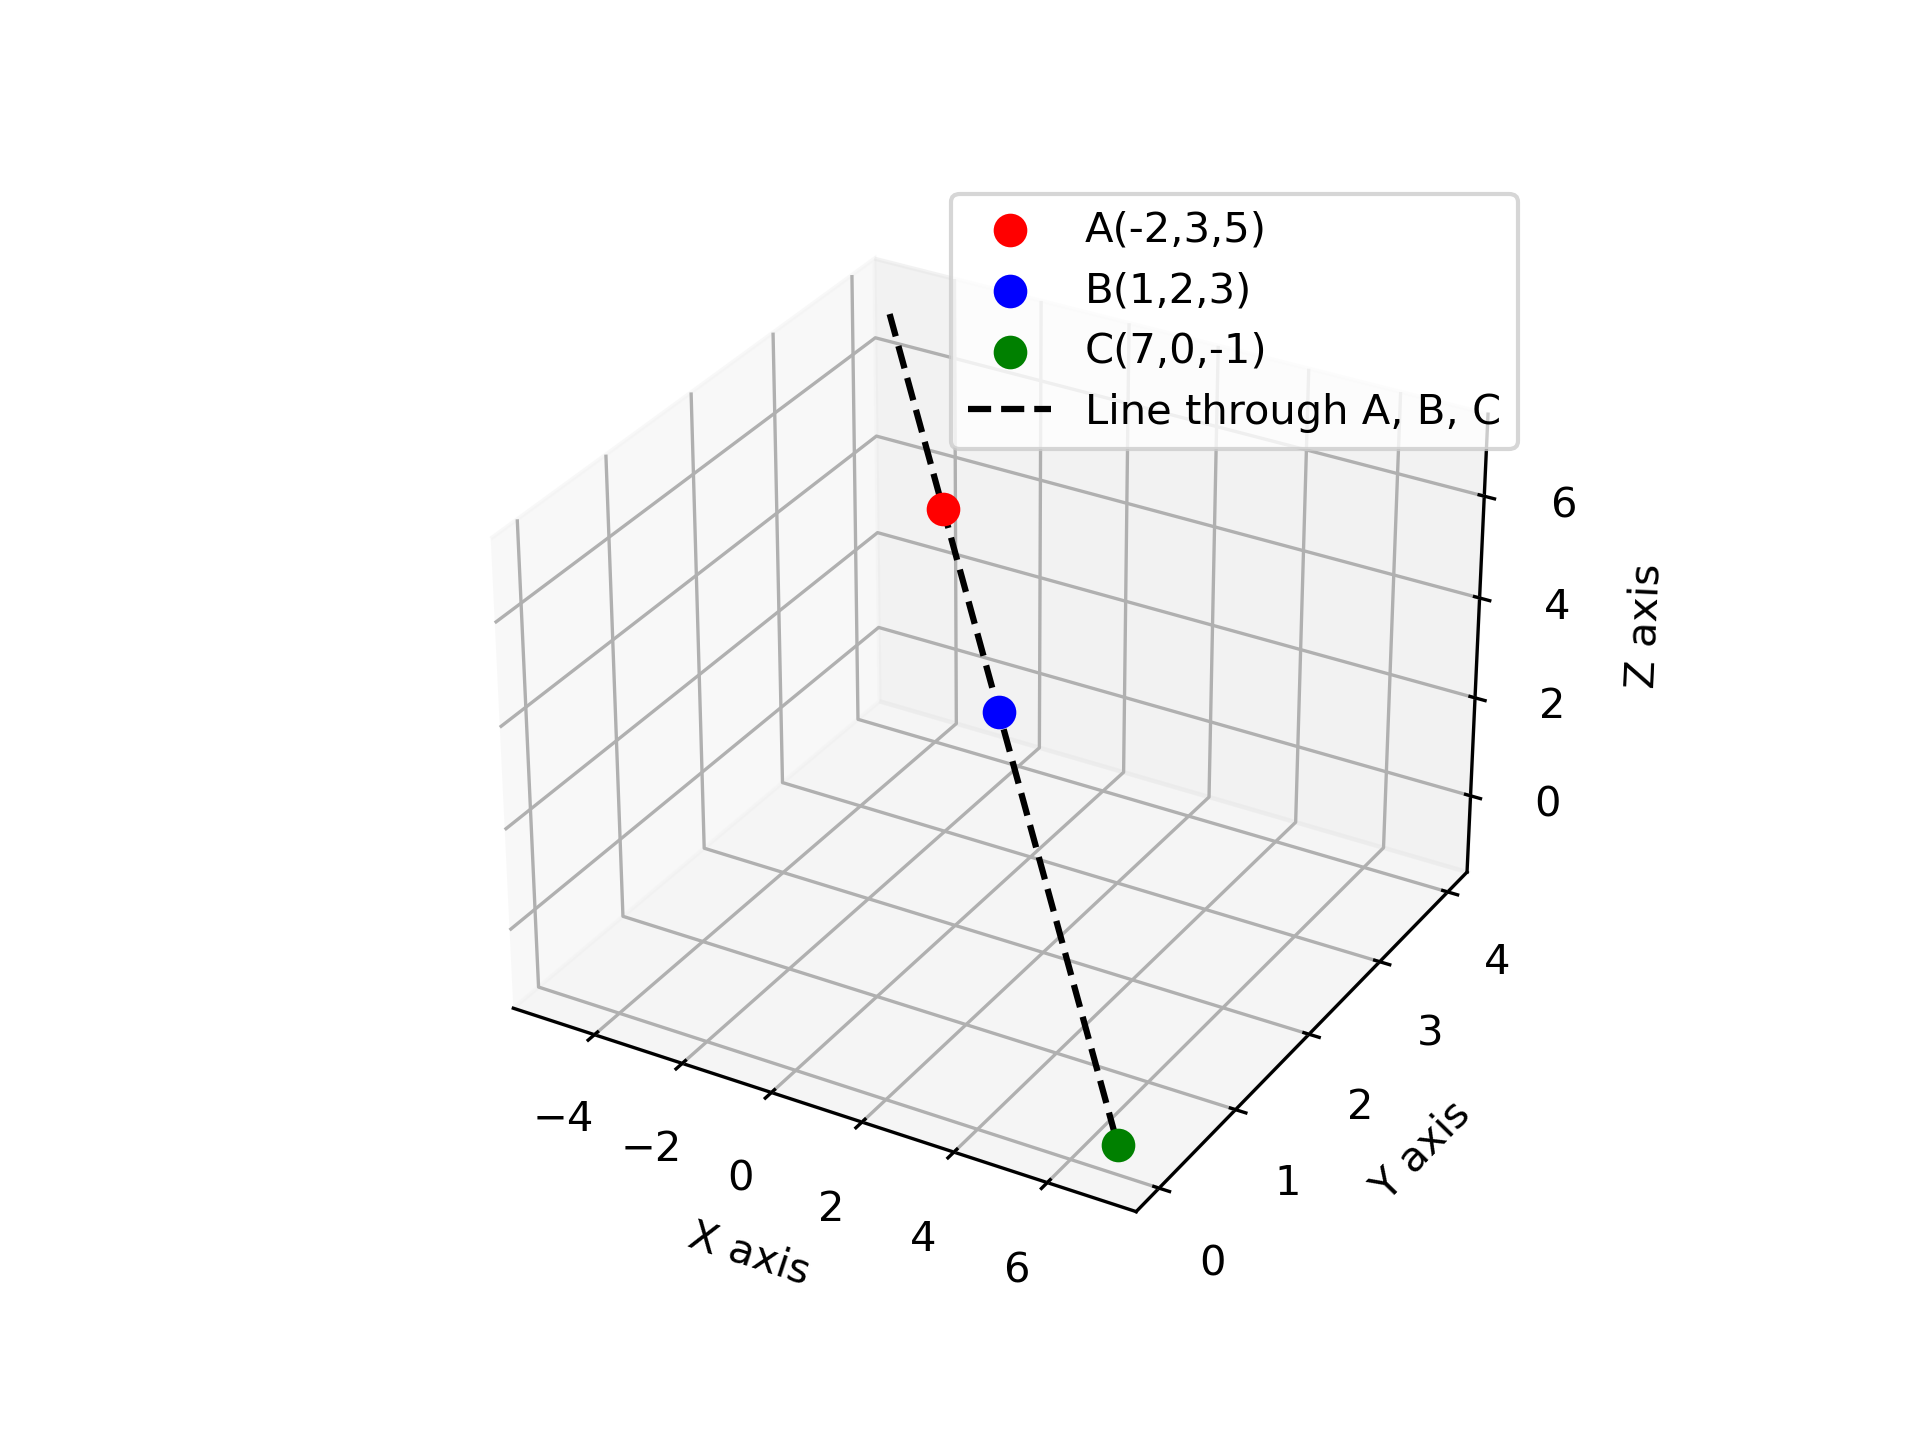
\includegraphics[width=0.7\linewidth]{/Users/unnathi/Documents/ee1030-2025/ai25btech11012/matgeo/1.11.14/figs/fig.png}
   \caption{}
   \label{stemplot}
\end{figure}





\end{document}
